% Options for packages loaded elsewhere
\PassOptionsToPackage{unicode}{hyperref}
\PassOptionsToPackage{hyphens}{url}
%
\documentclass[
  english,
  man]{apa6}
\usepackage{amsmath,amssymb}
\usepackage{lmodern}
\usepackage{ifxetex,ifluatex}
\ifnum 0\ifxetex 1\fi\ifluatex 1\fi=0 % if pdftex
  \usepackage[T1]{fontenc}
  \usepackage[utf8]{inputenc}
  \usepackage{textcomp} % provide euro and other symbols
\else % if luatex or xetex
  \usepackage{unicode-math}
  \defaultfontfeatures{Scale=MatchLowercase}
  \defaultfontfeatures[\rmfamily]{Ligatures=TeX,Scale=1}
\fi
% Use upquote if available, for straight quotes in verbatim environments
\IfFileExists{upquote.sty}{\usepackage{upquote}}{}
\IfFileExists{microtype.sty}{% use microtype if available
  \usepackage[]{microtype}
  \UseMicrotypeSet[protrusion]{basicmath} % disable protrusion for tt fonts
}{}
\makeatletter
\@ifundefined{KOMAClassName}{% if non-KOMA class
  \IfFileExists{parskip.sty}{%
    \usepackage{parskip}
  }{% else
    \setlength{\parindent}{0pt}
    \setlength{\parskip}{6pt plus 2pt minus 1pt}}
}{% if KOMA class
  \KOMAoptions{parskip=half}}
\makeatother
\usepackage{xcolor}
\IfFileExists{xurl.sty}{\usepackage{xurl}}{} % add URL line breaks if available
\IfFileExists{bookmark.sty}{\usepackage{bookmark}}{\usepackage{hyperref}}
\hypersetup{
  pdftitle={Reproduction of the Analysis of Holmes, To, \& Johnsrude (2021)},
  pdfauthor={Tiffany Hanratty1},
  pdflang={en-EN},
  pdfkeywords={Auditory perception, reproducibility, attention, speech perception, memory, learning},
  hidelinks,
  pdfcreator={LaTeX via pandoc}}
\urlstyle{same} % disable monospaced font for URLs
\usepackage{graphicx}
\makeatletter
\def\maxwidth{\ifdim\Gin@nat@width>\linewidth\linewidth\else\Gin@nat@width\fi}
\def\maxheight{\ifdim\Gin@nat@height>\textheight\textheight\else\Gin@nat@height\fi}
\makeatother
% Scale images if necessary, so that they will not overflow the page
% margins by default, and it is still possible to overwrite the defaults
% using explicit options in \includegraphics[width, height, ...]{}
\setkeys{Gin}{width=\maxwidth,height=\maxheight,keepaspectratio}
% Set default figure placement to htbp
\makeatletter
\def\fps@figure{htbp}
\makeatother
\setlength{\emergencystretch}{3em} % prevent overfull lines
\providecommand{\tightlist}{%
  \setlength{\itemsep}{0pt}\setlength{\parskip}{0pt}}
\setcounter{secnumdepth}{-\maxdimen} % remove section numbering
% Make \paragraph and \subparagraph free-standing
\ifx\paragraph\undefined\else
  \let\oldparagraph\paragraph
  \renewcommand{\paragraph}[1]{\oldparagraph{#1}\mbox{}}
\fi
\ifx\subparagraph\undefined\else
  \let\oldsubparagraph\subparagraph
  \renewcommand{\subparagraph}[1]{\oldsubparagraph{#1}\mbox{}}
\fi
% Manuscript styling
\usepackage{upgreek}
\captionsetup{font=singlespacing,justification=justified}

% Table formatting
\usepackage{longtable}
\usepackage{lscape}
% \usepackage[counterclockwise]{rotating}   % Landscape page setup for large tables
\usepackage{multirow}		% Table styling
\usepackage{tabularx}		% Control Column width
\usepackage[flushleft]{threeparttable}	% Allows for three part tables with a specified notes section
\usepackage{threeparttablex}            % Lets threeparttable work with longtable

% Create new environments so endfloat can handle them
% \newenvironment{ltable}
%   {\begin{landscape}\centering\begin{threeparttable}}
%   {\end{threeparttable}\end{landscape}}
\newenvironment{lltable}{\begin{landscape}\centering\begin{ThreePartTable}}{\end{ThreePartTable}\end{landscape}}

% Enables adjusting longtable caption width to table width
% Solution found at http://golatex.de/longtable-mit-caption-so-breit-wie-die-tabelle-t15767.html
\makeatletter
\newcommand\LastLTentrywidth{1em}
\newlength\longtablewidth
\setlength{\longtablewidth}{1in}
\newcommand{\getlongtablewidth}{\begingroup \ifcsname LT@\roman{LT@tables}\endcsname \global\longtablewidth=0pt \renewcommand{\LT@entry}[2]{\global\advance\longtablewidth by ##2\relax\gdef\LastLTentrywidth{##2}}\@nameuse{LT@\roman{LT@tables}} \fi \endgroup}

% \setlength{\parindent}{0.5in}
% \setlength{\parskip}{0pt plus 0pt minus 0pt}

% \usepackage{etoolbox}
\makeatletter
\patchcmd{\HyOrg@maketitle}
  {\section{\normalfont\normalsize\abstractname}}
  {\section*{\normalfont\normalsize\abstractname}}
  {}{\typeout{Failed to patch abstract.}}
\patchcmd{\HyOrg@maketitle}
  {\section{\protect\normalfont{\@title}}}
  {\section*{\protect\normalfont{\@title}}}
  {}{\typeout{Failed to patch title.}}
\makeatother
\shorttitle{Voice Familiarity}
\keywords{Auditory perception, reproducibility, attention, speech perception, memory, learning }
\DeclareDelayedFloatFlavor{ThreePartTable}{table}
\DeclareDelayedFloatFlavor{lltable}{table}
\DeclareDelayedFloatFlavor*{longtable}{table}
\makeatletter
\renewcommand{\efloat@iwrite}[1]{\immediate\expandafter\protected@write\csname efloat@post#1\endcsname{}}
\makeatother
\usepackage{lineno}

\linenumbers
\usepackage{csquotes}
\ifxetex
  % Load polyglossia as late as possible: uses bidi with RTL langages (e.g. Hebrew, Arabic)
  \usepackage{polyglossia}
  \setmainlanguage[]{english}
\else
  \usepackage[main=english]{babel}
% get rid of language-specific shorthands (see #6817):
\let\LanguageShortHands\languageshorthands
\def\languageshorthands#1{}
\fi
\ifluatex
  \usepackage{selnolig}  % disable illegal ligatures
\fi
\newlength{\cslhangindent}
\setlength{\cslhangindent}{1.5em}
\newlength{\csllabelwidth}
\setlength{\csllabelwidth}{3em}
\newenvironment{CSLReferences}[2] % #1 hanging-ident, #2 entry spacing
 {% don't indent paragraphs
  \setlength{\parindent}{0pt}
  % turn on hanging indent if param 1 is 1
  \ifodd #1 \everypar{\setlength{\hangindent}{\cslhangindent}}\ignorespaces\fi
  % set entry spacing
  \ifnum #2 > 0
  \setlength{\parskip}{#2\baselineskip}
  \fi
 }%
 {}
\usepackage{calc}
\newcommand{\CSLBlock}[1]{#1\hfill\break}
\newcommand{\CSLLeftMargin}[1]{\parbox[t]{\csllabelwidth}{#1}}
\newcommand{\CSLRightInline}[1]{\parbox[t]{\linewidth - \csllabelwidth}{#1}\break}
\newcommand{\CSLIndent}[1]{\hspace{\cslhangindent}#1}

\title{Reproduction of the Analysis of Holmes, To, \& Johnsrude (2021)}
\author{Tiffany Hanratty\textsuperscript{1}}
\date{}


\authornote{

Tiffany Hanratty, Department of Psychology, Brooklyn College.

Correspondence concerning this article should be addressed to Tiffany Hanratty, 2900 Bedford Ave. E-mail: \href{mailto:TIFFANY.HANRATTY66@bcmail.cuny.edu}{\nolinkurl{TIFFANY.HANRATTY66@bcmail.cuny.edu}}

}

\affiliation{\vspace{0.5cm}\textsuperscript{1} Brooklyn College}

\abstract{
This semester project works to recreate the statistical analysis portion of a study by Holmes, To, \& Johnsrude (2012). This analysis was run on the training portion of the study. Three paired t-tests were used to analyze the data in order to help determine significance when comparing different groups. The training portion of this paper analyzes 3 groups: the most familiar condition, the moderately familiar condition, and the least familiar condition (Holmes, To, and Johnsrude, 2021).
}



\begin{document}
\maketitle

The authors of this study examined how different lengths of voice exposure relate to voice intelligibility and voice recognition (Holmes, To, \& Johnsrude, 2021). The study consisted of 50 adult participants, and was broken up into four different parts. This data reanalysis is focused on the training portion of this study. The training portion analyses voice recognition performance in three categorize: most familiar, moderately familiar, and least familiar voice. Information on the sections regarding familiarization, the explicit-recognition test, and the speech-intelligibility test can be found in the complete study by Holmes, To, \& Johnsrude (2021).
The data for this analysis reduction can be found at, and were downloaded from \url{https://osf.io/7kdyc/}.

\hypertarget{methods}{%
\section{Methods}\label{methods}}

\hypertarget{participants}{%
\subsection{Participants}\label{participants}}

This experiment contained a total of 50 participants which were all aged 18 to 28 (Holmes, To, \& Johnsrude, 2021).

\hypertarget{material}{%
\subsection{Material}\label{material}}

Details pertaining to the acoustic stimuli used in this experiment can be found in the study conducted by Holmes, To, \& Johnsrude (2021).

\hypertarget{procedure}{%
\subsection{Procedure}\label{procedure}}

This experiment consisted of familiarization, training, an explicit-recognition test, and a speech-intelligibility test (Holmes, To, and Johnsrude, 2021). This reanalysis pertains to the training portion of this study. The training portion of this study consisted of participants hearing multiple sentences which could be spoken in one of three categories, most familiar, moderately familiar, or least familiar. Some participants (N = 25) heard training sentences alone, while other participants (N = 25) heard the sentences with background noise in the form of babbling. Participants were asked after each sentence to choose the name of the speaker of the sentence, which corresponds to the familiarity category. Participants were provided with immediate feedback as to whether or not they were correct. Detailed information on the remaining three sections of this study can be found in Holmes, To, \& Johnsrude (2021).

\hypertarget{results}{%
\section{Results}\label{results}}

\begin{verbatim}
## function (dir) 
## .Internal(setwd(dir))
## <bytecode: 0x0000000012be9e58>
## <environment: namespace:base>
\end{verbatim}

\begin{verbatim}
## 
##  Paired t-test
## 
## data:  all_data$fam_1 and all_data$fam_2
## t = 4.2875, df = 49, p-value = 8.447e-05
## alternative hypothesis: true difference in means is not equal to 0
## 95 percent confidence interval:
##  2.036763 5.630437
## sample estimates:
## mean of the differences 
##                  3.8336
\end{verbatim}

\begin{verbatim}
## 
##  Paired t-test
## 
## data:  all_data$fam_1 and all_data$fam_3
## t = 3.5619, df = 49, p-value = 0.0008311
## alternative hypothesis: true difference in means is not equal to 0
## 95 percent confidence interval:
##  1.709717 6.136283
## sample estimates:
## mean of the differences 
##                   3.923
\end{verbatim}

\begin{verbatim}
## 
##  Paired t-test
## 
## data:  all_data$fam_2 and all_data$fam_3
## t = 0.15586, df = 49, p-value = 0.8768
## alternative hypothesis: true difference in means is not equal to 0
## 95 percent confidence interval:
##  -1.063256  1.242056
## sample estimates:
## mean of the differences 
##                  0.0894
\end{verbatim}

\begin{tabular}{l|l|r|r}
\hline
value & name & meanRT & SEMRT\\
\hline
1 & fam & 98.2568 & 0.2078432\\
\hline
2 & fam & 94.4232 & 1.0142461\\
\hline
3 & fam & 94.3338 & 1.1859128\\
\hline
\end{tabular}

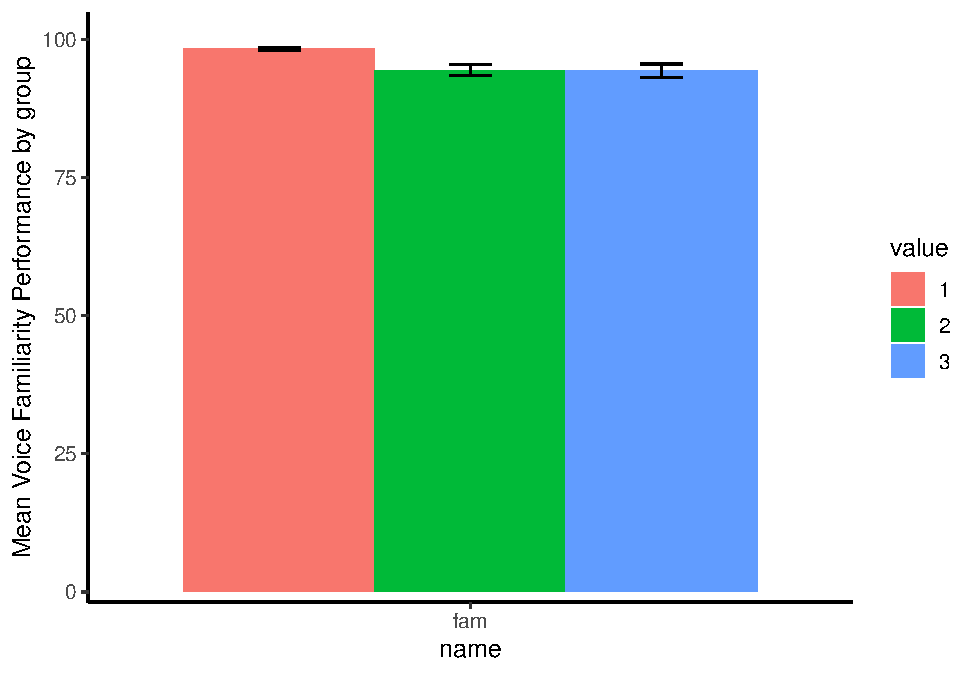
\includegraphics{APAreport_files/figure-latex/unnamed-chunk-5-1.pdf}

\hypertarget{hand-reporting}{%
\subsection{Hand Reporting}\label{hand-reporting}}

A paired t-test was used to compare familiarity conditions with performance. Better performance was seen in the most familiar condition compared to the moderately familiar condition, t(49) = 4.29, p \textless{} .001 (Holmes, To, and Johnsrude, 2021). There was also better performance seen in the most familiar condition compared to the least familiar condition, t(49) = 3.56, p = .001 (Holmes, To, and Johnsrude, 2021). There was not a significant difference found in the moderately familiar group compared to the least familiar group, t(49) = 0.16, p = .88. The confidence interval values were not able to be reproduced in this reanalysis.

\hypertarget{papaja-reporting}{%
\subsection{Papaja Reporting}\label{papaja-reporting}}

A paired t-test was used to compare familiarity conditions with performance. Better performance was seen in the most familiar condition compared to the moderately familiar condition, \(M_d = 3.83\), 95\% CI \([2.04\), \(5.63]\), \(t(49) = 4.29\), \(p < .001\) (Holmes, To, and Johnsrude, 2021). There was also better performance seen in the most familiar condition compared to the least familiar condition, \(M_d = 3.92\), 95\% CI \([1.71\), \(6.14]\), \(t(49) = 3.56\), \(p = .001\) (Holmes, To, and Johnsrude, 2021). There was not a significant difference found in the moderately familiar group compared to the least familiar group, \(M_d = 0.09\), 95\% CI \([-1.06\), \(1.24]\), \(t(49) = 0.16\), \(p = .877\). The confidence interval values were not able to be reproduced in this reanalysis.

\hypertarget{discussion}{%
\section{Discussion}\label{discussion}}

The analysis which was reported by Holmes, To, \& Johnsrude (2021) was partially successfully reproduced in this reanalysis. Both the t-test values and the p-values in this reanalysis match the reported values in Holmes, To, \& Johnsrude (2021). The confidence interval values were not able to be replicated in this reanalysis. A simulation based power analysis will be completed in the following section.

\hypertarget{simulation-based-power-analysis}{%
\subsection{Simulation-based power analysis}\label{simulation-based-power-analysis}}

This study ran three t-tests comparing performance between different groups of voice familiarity. The t-tests consisted of performance comparison between the most familiar voice compared to a moderately familiar voice, the most familiar voice compared to the least familiar voice, and the moderately familiar voice compared to the least familiar voice.

This power analysis was conducted in RStudio. For this power analysis a variable was generated in order to indicate the possible occurring effect sizes in this study. A simulation was run for each possible effect size using 1000 simulated experiments. Values were sampled using an approximately normal distribution. The replicated values' mean is set to be equal to the effect size. Fifty values were run for this distribution to emulate the fifty participants in the experiment. Every time this simulated test is conducted, a p-value is measured. This test will then analyze how many times these simulated experiments produced a p-value at a significance value of p \textless{} 0.05.

Based on the findings of this power curve, when the effect size is at approximately 0.7, a design similar to this studies design will detect an effect at p \textless{} 0.05 close to 100\% of the time. If the power of a study needs to be increased, a relatively simple way to increase statistical power would be to increase the sample size.

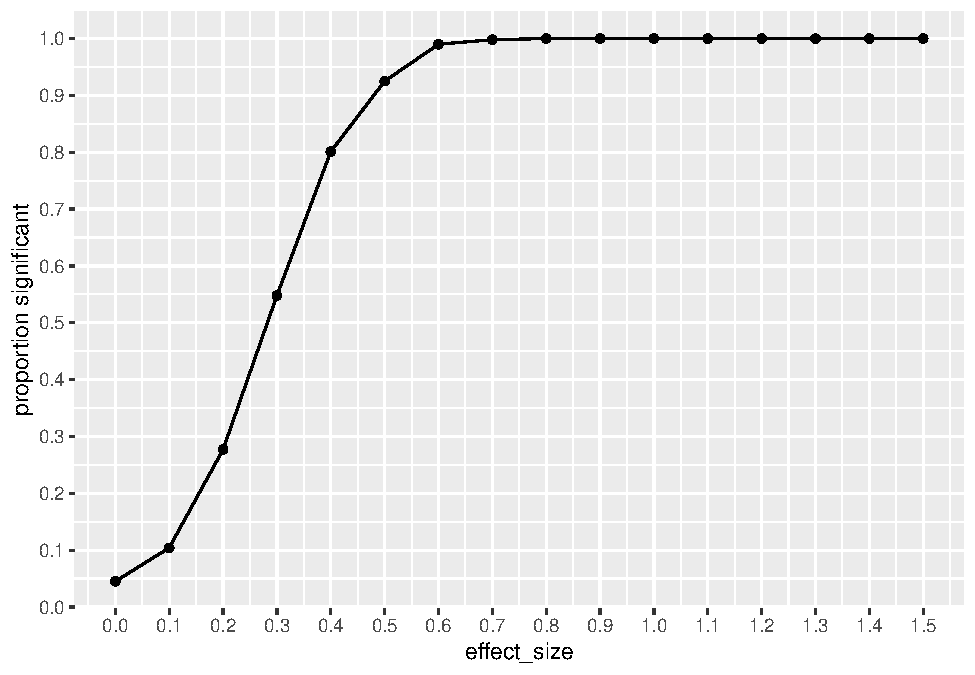
\includegraphics{APAreport_files/figure-latex/unnamed-chunk-6-1.pdf}

\newpage

\hypertarget{references}{%
\section{References}\label{references}}

Holmes, E., To, G., \& Johnsrude, I. S. (2021). How Long Does
It Take for a Voice to Become Familiar? Speech
Intelligibility and Voice Recognition Are Differentially
Sensitive to Voice Training. Psychological science, 32(6),
903--915. \url{https://doi.org/10.1177/0956797621991137}

\begingroup
\setlength{\parindent}{-0.5in}
\setlength{\leftskip}{0.5in}

\hypertarget{refs}{}
\begin{CSLReferences}{0}{0}
\end{CSLReferences}

\endgroup


\end{document}
